\documentclass[11pt]{article}

% ---------------------------------------------------------------------------
% WORKSHOP / arXiv preprint draft -- SKELETON ONLY (prose to be authored).
% Swap \documentclass for the venue style file once a target is chosen.
% Story (LOCKED 2026-06-08):
%   Headline   : WE WIN -- the cheapest spectral-polar member is the fastest
%                LoRA optimizer.
%   Protagonist: coupled two-sided DIAGONAL curvature + full polar + op-norm radius
%                (kl-diag-polar-lora).
%   Claim      : it matches the expensive members and beats AdamW 1.2-1.7x
%                across 9 (model,dataset,rank) settings -- the expensive
%                machinery is dead weight.
% ---------------------------------------------------------------------------

\usepackage{amssymb,amsmath,amsthm,amsbsy,amsfonts}
\usepackage{mathtools}
\usepackage[letterpaper,margin=1in]{geometry}
\usepackage{bm}
\usepackage{graphicx}
\usepackage{booktabs}
\usepackage{algorithm}
\usepackage{algpseudocode}
% Looser line spacing inside algorithm blocks for readability.
\makeatletter
\newcommand{\algspacing}{\setlength{\@tempdima}{0pt}\renewcommand{\baselinestretch}{1.25}\selectfont}
\makeatother
\algrenewcommand\algorithmicrequire{\textbf{Input:}}
% Phase header: blank line + vertical space above, bold label.
\algnewcommand\algorithmicphase{\vspace{5pt}\textbf}
\algnewcommand\Phase{\Statex\algorithmicphase}
\usepackage{enumitem}
\usepackage{xcolor}
\usepackage[colorlinks,citecolor=blue,urlcolor=blue]{hyperref}
\usepackage[nameinlink]{cleveref}
\usepackage[firstinits=true,backend=bibtex,style=numeric-comp,citestyle=numeric-comp,sorting=nyt,url=false,arxiv=false,isbn=false,doi=false]{biblatex}
\bibliography{references}

\graphicspath{{figs/}}

% --- macros -----------------------------------------------------------------
\renewcommand{\vec}[1]{\bm{#1}}
\newcommand{\mat}[1]{\bm{#1}}
\newcommand{\R}{\mathbb{R}}
\newcommand{\E}{\mathbb{E}}
\DeclareMathOperator{\diag}{diag}
\DeclareMathOperator*{\argmin}{arg\,min}
\DeclareMathOperator*{\argmax}{arg\,max}
\newcommand{\smax}{\sigma_{\max}}
\newcommand{\DW}{\Delta W}
\newcommand{\polar}{\varphi}                 % polar map  U\Sigma V^T -> U V^T
% Working method name -- rename in one place once finalized.
\newcommand{\methodname}{\textsc{Polar-LoRA}\xspace}
\usepackage{xspace}
% Visible marker for numbers pending the full-polar confirm/negate sweep.
\newcommand{\PLACEHOLDER}[1]{\textcolor{red}{[#1]}}
% theorem environments
\theoremstyle{plain}
\newtheorem{lemma}{Lemma}
\newtheorem{proposition}{Proposition}
\newtheorem{corollary}{Corollary}
\theoremstyle{definition}
\newtheorem{definition}{Definition}
\theoremstyle{remark}
\newtheorem{remark}{Remark}

\title{\methodname}  % working title -- revisit before submission
\author{}
\date{}

\begin{document}
\maketitle

% ===========================================================================
\begin{abstract}
We introduce \methodname{}, a LoRA optimizer that applies a polar (spectral-cap)
map to two-sided-whitened momentum and sizes each step by a per-factor
operator-norm radius. Spectral and curvature-aware updates reach a target loss in
fewer steps than AdamW on full-weight training, but carrying them to the LoRA
factors $A,B$ is not straightforward: a per-factor polar depends on the
$\DW{=}BA$ factorization rather than on $\DW$ itself, the factor norms can diverge,
and the known remedies appear only bundled into heavy methods, leaving it unclear
which ingredient carries the gain. \methodname{} keeps only the cheap essential
parts --- a coupled two-sided \emph{diagonal} curvature whitener, a full polar
(PolarExpress), and an operator-norm step radius
$\rho=\eta/(\smax(A){+}\smax(B))$. Across $9$ (model, dataset, rank) settings
spanning $4$ base models and $3$ corpora, it reaches AdamW's eval loss in
$1.2$--$1.7\times$ fewer steps, and ablations show that the more expensive
Kronecker-factored curvature and inner-iteration refinement are unnecessary. The
per-step overhead is $\le 6\%$ at production batch and the optimizer state is
${\approx}\tfrac12$ AdamW's, so the step-count speedup survives in wall-clock.
\end{abstract}

% ===========================================================================
\section{Introduction}
\label{sec:intro}
% Hard limits: <= 1.5 pages; methods by page 2-3; 2-4 contribution bullets <=2 lines.
%
% Citation keys (verify entries in references.bib against arXiv before submission):
%   kang_specgf=2602.06385, imuon=2605.09238, spectron=2602.12429,
%   soap=2409.11321, adaprelora=2605.08734, mua=2602.06204,
%   polarexpress=2505.16932, muon=<verify>,
%   lorarite=2410.20625 (ICLR'25, published -- NOT concurrent),
%   loramuon=2606.12921 (concurrent, 2026-06-11), loraalpha=2606.12883 (concurrent).

Low-rank adaptation (LoRA) is the default way to fine-tune a large language model:
it freezes the pretrained weight $W_0$ and learns a rank-$r$ adapter
$\DW=(\alpha/r)\,BA$ with $A\in\R^{r\times d_{\mathrm{in}}}$,
$B\in\R^{d_{\mathrm{out}}\times r}$. Which optimizer trains that adapter is an
under-examined lever: practice defaults to AdamW --- the optimizer for dense
weights --- applied unchanged to the factors $A,B$.

On full-weight training, two families reach a target loss in fewer steps than
AdamW: spectral / steepest-descent updates (the Muon family) and Shampoo-style
curvature whitening. Neither carries cleanly to the LoRA factors. The product
$\DW=BA$ is invariant under $(A,B)\mapsto(NA,BN^{-1})$ for invertible $N$, but a
per-factor polar map is not --- so it depends on the chosen factorization rather
than on $\DW$ --- and the factor norms can diverge under the corresponding flow
\cite{kang_specgf, imuon}.

Remedies exist, but each is partial and bundled with expensive machinery. The
invariance fix --- LoRA-RITE \cite{lorarite}, then iMuon \cite{imuon} and the
concurrent LoRA-Muon \cite{loramuon} --- whitens each factor by its partner's Gram
root, but controls only the merged \emph{product} step and leaves the per-factor
step unbounded. A per-factor operator-norm radius exists (Spectron
\cite{spectron}), but for native low-rank \emph{pretraining}, not adapter
fine-tuning. Two-sided curvature exists (Shampoo/SOAP \cite{soap}, AdaPreLoRA
\cite{adaprelora}), but without a spectral cap and, for AdaPreLoRA, at a cost that
scales with the dense weight. No single method has the cheap union of all three,
and it is unclear which ingredient carries the speedup.

\methodname{} assembles that union and ablates the expensive parts away. One step
is: bias-corrected momentum $\to$ whiten each factor in a learned two-sided
\emph{diagonal} curvature metric $\to$ full polar (spectral cap) $\to$ re-pin the
magnitude to a per-factor operator-norm radius $\rho=\eta/(\smax(A){+}\smax(B))$.
The radius bounds the merged step independent of the factor conditioning, which
lets the method train from the standard $B{=}0$ init where the partner-Gram core
cannot.

\paragraph{Contributions.}
\begin{itemize}[leftmargin=1.5em,itemsep=2pt,topsep=2pt]
  \item \textbf{A fast, cheap LoRA optimizer.} \methodname{} reaches AdamW's eval
        loss in $1.2$--$1.7\times$ fewer steps across $9$ (model, dataset, rank)
        settings, at $\le 6\%$ per-step wall overhead and ${\approx}\tfrac12$
        AdamW's optimizer state.
  \item \textbf{Operator-norm magnitude control.} A per-factor operator-norm radius
        bounds the merged step, so the method trains from the standard $B{=}0$ init
        where the partner-Gram family cannot, and wins at every rank
        $r\in\{32,64,128,256\}$. Its loss-minimizing learning rate stays fixed
        across these ranks while AdamW's drifts (\Cref{fig:lr_transfer}).
  \item \textbf{What carries the gain.} Ablations show that the cheap two-sided
        \emph{diagonal} whitener is necessary, but the more expensive
        Kronecker-factored curvature (Shampoo/SOAP \cite{soap}, KL-Shampoo
        \cite{klshampoo}) and inner-iteration refinement are not; the polar cap
        follows the spectral-method literature \cite{imuon, spectron, polarexpress}.
  \item \textbf{A LoRA-optimizer benchmark.} A $9$-setting comparison under a
        speedup-to-AdamW metric over $4$ base models and $3$ corpora.
\end{itemize}

The speedup is task-dependent --- largest out-of-distribution and at higher rank
($1.30\times$ on in-distribution code versus $1.73\times$ on an out-of-distribution
corpus, at the same model and rank) --- and the per-step overhead is small enough
that it survives in wall-clock.

% ===========================================================================
\section{Setup and metric}
\label{sec:setup}
\paragraph{LoRA.} We adapt each frozen base weight $W_0$ with
$\DW=(\alpha/r)\,BA$, $A\in\R^{r\times d_{\mathrm{in}}}$,
$B\in\R^{d_{\mathrm{out}}\times r}$, $\alpha{=}r$, on all linear modules, from the
standard $B{=}0$ initialization.

\paragraph{Held-fixed protocol.} Every optimizer comparison fixes the base model,
dataset and split, rank and $\alpha$, target modules, sequence length, batch size,
gradient accumulation, dtype, and a constant learning rate with no warmup or decay;
only the optimizer and its learning rate vary. We select the learning rate per
(optimizer, setting) on held-out eval loss over a fixed grid.

\paragraph{Speedup metric.} For a setting with horizon $H$ steps, let
$\ell^\star$ be AdamW's best-learning-rate final eval loss. The \emph{speedup} of a
method is $H/s$, where $s$ is the first (interpolated) step at which the method's
best-learning-rate trajectory reaches $\ell^\star$. A $1.5\times$ speedup means the
method matches AdamW's final loss in two-thirds of the steps; a method that never
reaches $\ell^\star$ within the horizon has no speedup. All results are single seed
(\Cref{sec:limitations}).

% ===========================================================================
\section{Method: \methodname}
\label{sec:method}
% MAIN STORY (outlined): the per-step DIRECTION of all three is the linear-minimization
% oracle (LMO) of the gradient under a norm -- 3.1 spectral norm per factor, 3.2 partner-Gram
% product norm, 3.3 learned two-sided diagonal-curvature metric. OURS IS NOT A PURE LMO:
% the metric P,Q is a coupled diagonal KL flip-flop (estimation, not an LMO), and the
% MAGNITUDE is the operator-norm pin rho=eta/(smax A+smax B) (a separate rule, not the LMO
% budget tau). Keep those three ingredients distinct in the prose.
% Prose is terse here by design (author expands); the equations are the content.
% Citation keys (verify in references.bib): kang_specgf, imuon, spectron,
% polarexpress, soap, mua, tilde_csd (compositional steepest descent -- no arXiv).

% --- setup + the steepest-descent (LMO) view (MAIN STORY) ---------------------
% All three updates are the same step (steepest descent under a norm) under
% different norms. Statements in body; proofs in \Cref{app:proofs}.
\paragraph{Setup.}
\begin{itemize}[leftmargin=1.5em,itemsep=1pt,topsep=2pt]
  \item LoRA factors $A\in\R^{r\times d_{\mathrm{in}}}$, $B\in\R^{d_{\mathrm{out}}\times r}$; adapter $\DW=(\alpha/r)\,BA$.
  \item $G\triangleq\partial L/\partial(BA)$: gradient of the loss w.r.t.\ the \emph{unscaled} product $BA$ (the $\alpha/r$ scale is absorbed into the learning rate $\eta>0$). Per-factor gradients $G_A=B^\top G$, $G_B=GA^\top$.
  \item $\dot A,\dot B$: the updates applied to the factors ($A\leftarrow A+\dot A$).
  \item $\polar(M)=UV^\top$ for the SVD $M=U\Sigma V^\top$ (sets each nonzero singular value to $1$); spectral norm $\|M\|_2=\smax(M)$; $\langle X,Y\rangle=\operatorname{tr}(X^\top Y)$; Gram matrices $S_A=AA^\top$, $S_B=B^\top B$.
\end{itemize}
\textbf{Steepest descent under a norm} (the LMO), for a factor gradient $M$ and a norm $\|\cdot\|$, is the update
\begin{equation}
  \eta\,\argmin_{\|U\|\le1}\langle M,U\rangle .
  \label{eq:lmo}
\end{equation}
The three variants specialize $\|\cdot\|$ to three different norms; \Cref{lem:lmo} is the case of the spectral norm $\|\cdot\|_2$.

\subsection{Naive Muon on the factors}
\label{sec:method-naive}
\paragraph{Norm.} The spectral norm $\|\cdot\|_2$, applied to each factor separately.
\begin{lemma}[Spectral-norm LMO]\label{lem:lmo}
$-\polar(M)\in\argmin_{\|U\|_2\le1}\langle M,U\rangle$ for any matrix $M$ (uniquely so when $M$ has full rank with distinct singular values). \emph{(\Cref{app:proofs}.)}
\end{lemma}
\noindent Applying \Cref{lem:lmo} to each factor gradient:
\begin{equation}
  \dot A=-\eta\,\polar(G_A),\qquad \dot B=-\eta\,\polar(G_B).
  \label{eq:naive}
\end{equation}
Two defects on a factored weight:
\begin{itemize}[leftmargin=1.5em,itemsep=1pt,topsep=2pt]
  \item \emph{Factorization-dependent.} The product $\DW=BA$ is invariant under $(A,B)\mapsto(NA,BN^{-1})$ for invertible $N$, but the factor gradient transforms as $G_A\mapsto N^{-\top}G_A$. Since $\polar$ is not equivariant, \eqref{eq:naive} depends on the factorization, not on $\DW$ alone \cite{imuon}.
  \item \emph{Unbounded merged step.} The merged step
        $\|B\dot A+\dot B A\|_2\le\eta\big(\|A\|_2+\|B\|_2\big)$
        grows with the factor norms, which can diverge under the corresponding flow \cite{kang_specgf}.
\end{itemize}

\subsection{iMuon / compositional Muon}
\label{sec:method-imuon}
\paragraph{LMO (half-split).} Budget each factor's contribution to the product step separately --- the tractable surrogate \cite{tilde_csd} for the harder joint constraint $\|\dot B A+B\dot A\|_2\le\eta$:
\begin{equation}
  \min_{\dot A}\ \langle G_A,\dot A\rangle \ \ \text{s.t.}\ \ \|B\dot A\|_2\le\eta,
  \qquad
  \min_{\dot B}\ \langle G_B,\dot B\rangle \ \ \text{s.t.}\ \ \|\dot B A\|_2\le\eta .
  \label{eq:imuon-lmo}
\end{equation}
\begin{proposition}[Partner-Gram step]\label{prop:imuon}
The solution of \eqref{eq:imuon-lmo} whitens each factor by its partner's Gram root:
\begin{equation*}
  \dot A=-\eta\,S_B^{-1/2}\,\polar\!\big(S_B^{-1/2}G_A\big),\qquad
  \dot B=-\eta\,\polar\!\big(G_B S_A^{-1/2}\big)\,S_A^{-1/2}.
\end{equation*}
\emph{(\Cref{app:proofs}; iMuon \cite{imuon}, and the half-split of compositional Muon \cite{tilde_csd}.)}
\end{proposition}
\begin{corollary}[Product-step invariance]\label{cor:imuon}
$\|B\dot A\|_2=\eta$, independent of the factor norms --- so no runtime rescale is needed. \emph{(\Cref{app:proofs}.)}
\end{corollary}
\begin{itemize}[leftmargin=1.5em,itemsep=1pt,topsep=2pt]
  \item \emph{Same operator, other compositions.} Compositional Muon applies it to the attention products $W_QW_K^\top$ and $W_OW_V$ \cite{tilde_csd}.
  \item \emph{Same operator, three independent incarnations.} The memoryless core of LoRA-RITE \cite{lorarite} (moment accumulation stripped), iMuon's decoupled form \cite{imuon}, and the concurrent LoRA-Muon \cite{loramuon} all realize \Cref{prop:imuon}; \cite{loramuon} proves the RITE-core equivalence. Our ablation runs this shared core's \emph{direction} as the both-controls-removed arm, with the step magnitude pinned by the unit-spectral-norm rescale of \Cref{alg:ours} (\Cref{sec:exp}); the unpinned update's factor step is uncapped ($\propto1/\sigma_{\min}$ of the partner).
  \item \emph{The gap we close.} The raw factor step is uncontrolled --- $\|\dot A\|_2$ scales as $\eta/\sigma_{\min}(B)$ --- with no per-factor operator-norm radius to bound it.
\end{itemize}

\subsection{Ours: \methodname}
\label{sec:method-ours}
\paragraph{Motivation.} Naive Muon (\Cref{lem:lmo}) and iMuon (\Cref{prop:imuon}) are the same spectral LMO under the Euclidean inner product, differing only in what they cap. \methodname{} keeps a spectral LMO for the \emph{direction} but measures it in a learned two-sided metric, and sets the \emph{magnitude} by a separate rule. Three stages:
\begin{itemize}[leftmargin=1.7em,itemsep=1pt,topsep=2pt]
  \item[(A)] \emph{Metric.} Estimate diagonal $P,Q$ online as the Kronecker factors of the gradient second moment (matrix-normal MLE \cite{klshampoo}; \Cref{par:coupling}).
  \item[(B)] \emph{Direction.} Spectral-norm LMO of the loss in that metric --- a whiten--polar--unwhiten step (\Cref{prop:ours}).
  \item[(C)] \emph{Magnitude.} Discard the LMO budget; re-pin to the operator-norm radius (\Cref{eq:ours-prodcap}).
\end{itemize}
Stages (A) and (B) are separate problems --- estimation, then a step under the \emph{frozen} estimate --- composed by alternation, not one objective.

\paragraph{(A) The metric.} Equip weight space with the two-sided diagonal inner product
\begin{equation}
  \langle X,Y\rangle_{P,Q}=\operatorname{tr}(X^\top P\,Y\,Q),\qquad
  \|X\|_{P,Q}=\|P^{1/2}XQ^{1/2}\|_2,
  \label{eq:ours-metric}
\end{equation}
with $P=\diag(p)\succ0$ on the output side ($d_{\mathrm{out}}$) and $Q=\diag(q)\succ0$ on the input side ($d_{\mathrm{in}}$). $P,Q$ are diagonal Kronecker factors of the gradient \emph{second moment}, estimated online (decay $\beta_2$) by \eqref{eq:ours-klcoupling}; $P=Q=I$ recovers the Euclidean spectral case of \Cref{sec:method-naive,sec:method-imuon}. The spectral cap in this metric whitens by $P^{-1/2},Q^{-1/2}$ (\Cref{prop:ours}).

\paragraph{Estimating the metric.}
\label{par:coupling}
Model the weight gradient as matrix-normal, $G\sim\mathcal{MN}(0,P,Q)$ with diagonal $P,Q$ --- the Kronecker second-moment fit of \cite{klshampoo,soap}. We never form $G$, but $\mathcal{MN}$ is closed under the factor maps, so the per-factor gradients are two views of the same $(P,Q)$:
\begin{equation}
\begin{aligned}
  G_A=B^\top G &\sim\mathcal{MN}(0,\,C_A,\,Q), &\quad C_A&=B^\top P B,\\
  G_B=GA^\top  &\sim\mathcal{MN}(0,\,P,\,C_B), &\quad C_B&=A\,Q\,A^\top .
\end{aligned}
\label{eq:ours-closure}
\end{equation}
$G_A$ resolves $Q$ and $G_B$ resolves $P$; each diagonal is the conditional MLE of its view with the partner core (an $r\times r$ matrix formed from the diagonals, never stored) held fixed --- the matrix-normal flip-flop \cite{klshampoo,dutilleul}:
\begin{equation}
  q_j=\mathrm{EMA}\Big[\tfrac1r\,(G_A)_{:,j}^\top C_A^{-1}(G_A)_{:,j}\Big],\qquad
  p_i=\mathrm{EMA}\Big[\tfrac1r\,(G_B)_{i,:}\,C_B^{-1}(G_B)_{i,:}^\top\Big].
  \label{eq:ours-klcoupling}
\end{equation}
It is unbiased ($\E[G_A^\top C_A^{-1}G_A]=rQ$) and couples the sides through the cores ($C_A$ injects $P$, $C_B$ injects $Q$); $C_A=C_B=I$ would drop to two independent Adafactor diagonals. We run one $\beta_2$-EMA alternation per step.

\paragraph{(B) The step: spectral LMO in the frozen metric.} With $P,Q$ \emph{frozen} at their current estimate, cap the product step in the metric \eqref{eq:ours-metric} and maximize alignment with the gradient:
\begin{equation}
  \max_{\dot A}\ \langle B\dot A,\,-G\rangle
  \quad\text{s.t.}\quad
  \|B\dot A\|_{P,Q}\le\tau .
  \label{eq:ours-opt}
\end{equation}
This is the spectral LMO of \Cref{lem:lmo} in the $P,Q$ metric, with $P,Q$ from (A) held fixed. Whitening both sides by $P^{-1/2},Q^{-1/2}$ reduces it to the Euclidean spectral case, giving a closed form.
\begin{proposition}[Metric LMO]\label{prop:ours}
For $B$ of full column rank, the solution of \eqref{eq:ours-opt} is
\begin{equation*}
  \dot A = -\tau\,C_A^{-1/2}\,\polar\!\big(C_A^{-1/2}\,G_A\,Q^{-1/2}\big)\,Q^{-1/2},
  \qquad C_A=B^\top P B .
\end{equation*}
\end{proposition}
\medskip
\noindent \methodname{} uses \Cref{prop:ours} for the step \emph{direction} only, on the bias-corrected Nesterov momentum $\hat M_A$ in place of the gradient:
\begin{equation}
  W_A \;=\; C_A^{-1/2}\,\polar\!\big(C_A^{-1/2}\,\hat M_A\,Q^{-1/2}\big)\,Q^{-1/2},
  \label{eq:ours-lmo}
\end{equation}
with $W_B$ the mirror ($C_B=AQA^\top$).

\paragraph{(C) The magnitude: operator-norm radius.} Since $\polar(\cdot)$ has unit spectral norm, the magnitude of $W_A$ is an artifact of the whitening, not the LMO budget $\tau$ --- stage (B) fixes only the \emph{direction}. \Cref{alg:ours} \emph{discards} it and re-pins the step to the operator-norm radius $\rho=\eta/(\smax(A)+\smax(B))$ via $\dot A=-\rho\,W_A/\smax(W_A)$, which caps the merged step independent of conditioning:
\begin{equation}
  \|B\dot A+\dot B A\|_2\le\rho\big(\smax(A)+\smax(B)\big)=\eta .
  \label{eq:ours-prodcap}
\end{equation}
This is a second trust region, separate from (B): a Euclidean operator-norm cap on the merged step, not the $P,Q$ cap of \eqref{eq:ours-opt} (whose budget $\tau$ is discarded). It makes the method stable from the standard $B{=}0$ init (\Cref{rem:b0}).

\begin{remark}[Relation to AdaPreLoRA]
\Cref{prop:ours} caps the whitened step in operator norm, giving the polar; a Frobenius cap instead gives the linear solve $\dot A\propto C_A^{-1}G_A Q^{-1}$ --- AdaPreLoRA \cite{adaprelora}, the same projection without the spectral cap.
\end{remark}

\begin{algorithm}[t]
\caption{\methodname{} step for one LoRA pair $(A,B)$ at iteration $t$}
\label{alg:ours}
\begin{algorithmic}[1]
\Require gradients $G_A,G_B$; momenta $M_A,M_B$; diagonals $P,Q$; decays $\beta_1,\beta_2$; rate $\eta$
\Phase{Momentum (Nesterov, bias-corrected)}
\State $M_A\gets\beta_1 M_A+(1-\beta_1)G_A$;\quad $\hat M_A\gets\big(\beta_1 M_A+(1-\beta_1)G_A\big)/(1-\beta_1^{t})$ \Comment{mirror for $B$}
\Phase{Whiten, polar, unwhiten}
\State $C_A\gets B^\top P B$;\quad $C_B\gets A Q A^\top$ \Comment{$r\times r$}
\State $W_A\gets C_A^{-1/2}\,\polar\!\big(C_A^{-1/2}\hat M_A Q^{-1/2}\big)\,Q^{-1/2}$
\State $W_B\gets P^{-1/2}\,\polar\!\big(P^{-1/2}\hat M_B C_B^{-1/2}\big)\,C_B^{-1/2}$
\Phase{Operator-norm step}
\State $\rho\gets\eta/(\smax(A)+\smax(B))$
\State $A\gets A-\rho\,W_A/\smax(W_A)$;\quad $B\gets B-\rho\,W_B/\smax(W_B)$
\Phase{Metric update (flip-flop, one alternation)}
\State $Q_{jj}\gets\beta_2 Q_{jj}+\tfrac{1-\beta_2}{r}(G_A)_{:,j}^\top C_A^{-1}(G_A)_{:,j}$
\State $P_{ii}\gets\beta_2 P_{ii}+\tfrac{1-\beta_2}{r}(G_B)_{i,:}C_B^{-1}(G_B)_{i,:}^\top$
\end{algorithmic}
\end{algorithm}
\noindent Every $\smax(\cdot)$ is the guarded estimate of \Cref{alg:smax}, and every inverse-sqrt is relative-damped (\Cref{app:damping}).

\begin{remark}[Why the operator-norm step is safe at the standard $B{=}0$ initialization]
\label{rem:b0}
LoRA starts at $B{=}0$, where the partner-Gram polar of \Cref{prop:imuon} has no stable learning rate but the operator-norm step does.
\begin{itemize}[leftmargin=1.5em,itemsep=1pt,topsep=2pt]
  \item \textbf{The failure.} $\polar(S_B^{-1/2}G_A)$ has unit spectral norm however small $G_A$ is, and the outer $S_B^{-1/2}$ scales it by up to $1/\sigma_{\min}(B)$, so $\|\dot A\|_2\approx\eta/\sigma_{\min}(B)$ --- unbounded as $B\to0$, undefined at $B{=}0$. Renormalizing to a scale-free step removes the gradient's natural $\|G_A\|\propto\sigma(B)$ protection; lowering $\eta$ does not help (it slows $B$'s escape by the same factor it shrinks the spurious step). So the decoupled spectral update --- iMuon's closed form (Cor.\ 4.1), re-derived by LoRA-Muon \cite{loramuon}, equivalent to simplified LoRA-RITE \cite{lorarite} --- has no stable rate from this init (\Cref{sec:exp}).
  \item \textbf{The family's workarounds.} iMuon applies the metric LMO to a \emph{joint} product-space momentum $M=\dot M_BA+B\dot M_A$ (a different update, not the decoupled solution) and prepends warmup to grow $B$ off zero; LoRA-Muon trains from nonzero random factors and never enters the regime.
  \item \textbf{Ours needs neither.} The operator-norm step $\dot A=-\rho\,W_A/\smax(W_A)$ pins $\|\dot A\|_2=\rho$ at every conditioning; at $B{=}0$, $\rho=\eta/(\smax(A)+\smax(B))=\eta/\smax(A)$ with $A$ a full-scale random factor --- an ordinary step. The polar discards the gradient's magnitude and the rescale re-imposes the radius, so the step size is a property of the method, not the factor conditioning.
\end{itemize}
\end{remark}

\paragraph{Cost.} \methodname{} is \emph{lighter} than AdamW in memory and adds a small, batch-amortized compute overhead.
\begin{itemize}[leftmargin=1.5em,itemsep=1pt,topsep=2pt]
  \item \textbf{Memory.} Same first moment as AdamW, but AdamW's second moment is replaced by two curvature diagonals $P,Q$ --- a factor $r$ smaller. The $r\times r$ cores $C_A=B^\top PB$, $C_B=AQA^\top$ are formed on the fly (\Cref{alg:ours}), not stored, and the inverse-sqrt is eigh-free (no eigenbasis, no $d\times d$ state). Net state ${\approx}\tfrac12$ AdamW's (\Cref{tab:optstate}).
  \item \textbf{Compute.} Per pair: $8$ matmuls of cost ${\sim}r^2d$ (the two cores, whiten/un-whiten, two curvature applies), two full polars (PolarExpress \cite{polarexpress}, PE${=}8$), two gram--Newton--Schulz inverse-sqrts \cite{gram_ns} (${\sim}r^3$). All $r\times r$ or $r\times d$, eigh-free; the polars dominate.
  \item \textbf{Wall.} Near-free at production batch: the fixed \texttt{optimizer.step} amortizes against the batch-scaling forward/backward (\Cref{sec:exp-walltime}).
\end{itemize}
\begin{table}[h]
\centering\small
\begin{tabular}{lccc}
\toprule
optimizer state (fp32) & floats / pair & Llama-3-8B & OLMo-2-1B \\
\midrule
AdamW         & $2r(d_{\mathrm{in}}{+}d_{\mathrm{out}})$     & $5.37$\,GB & $1.54$\,GB \\
\methodname{} & $(r{+}1)(d_{\mathrm{in}}{+}d_{\mathrm{out}})$ & $2.69$\,GB & $0.77$\,GB \\
\bottomrule
\end{tabular}
\caption{Optimizer state at $r{=}256$, all-linear LoRA: \methodname{} keeps AdamW's first moment but replaces the second moment with two $r{\times}$-smaller diagonals $P,Q$, ${\approx}\tfrac12$ AdamW's state ($671$M LoRA params for Llama-3-8B, $193$M for OLMo-2-1B).}
\label{tab:optstate}
\end{table}

% ===========================================================================
\section{Experiments}
\label{sec:exp}

\subsection{Main result: speedup across nine settings}
\methodname{} is faster than AdamW on every setting we tried.
\Cref{fig:hero} shows the showcase cell; \Cref{tab:speedup} reports the speedup at
all nine.

\begin{figure}[t]
  \centering
  
\includegraphics[width=0.72\linewidth]{fig1_hero.pdf}
  \caption{\textbf{\methodname{} reaches AdamW's loss in fewer steps.} Held-out eval
  loss versus training step on the showcase setting (Llama-3.2-1B,
  OpenMathInstruct-2, $r{=}256$, $9000$ steps), each method at its best learning
  rate. The dashed line marks AdamW's final loss; \methodname{} reaches it near step
  $5500$ --- a $1.63\times$ step speedup --- while iMuon does not reach it within the
  horizon. Single seed.}
  \label{fig:hero}
\end{figure}

\begin{table}[t]
  \centering\small
  \begin{tabular}{l r r r r r}
\toprule
 & \multicolumn{2}{c}{AdamW} & \multicolumn{3}{c}{\methodname} \\
\cmidrule(lr){2-3}\cmidrule(lr){4-6}
model / dataset / rank & lr & final & lr & speedup & speedup (lr-avg) \\
\midrule
Qwen2.5-1.5B / Aya-Bengali / r=256 & 0.0001 & 0.4979 & 0.03 & 1.73$\times$ & 1.39$\times$ \\
Llama-3.2-1B / OpenMathInstruct-2 / r=256 & 0.0001 & 0.3823 & 0.01 & 1.63$\times$ & 1.40$\times$ \\
OLMo-2-1B / opc-sft-stage2 / r=256 & 0.0001 & 0.7524 & 0.03 & 1.61$\times$ & 1.26$\times$ \\
Llama-3.2-1B / opc-sft-stage2 / r=256 & 3e-05 & 0.6948 & 0.003 & 1.55$\times$ & 1.24$\times$ \\
Llama-3.2-1B / OpenMathInstruct-2 / r=64 & 0.0001 & 0.3991 & 0.01 & 1.54$\times$ & 1.25$\times$ \\
Llama-3.2-1B / OpenMathInstruct-2 / r=128 & 0.0001 & 0.3890 & 0.01 & 1.52$\times$ & 1.28$\times$ \\
Llama-3.2-1B / OpenMathInstruct-2 / r=32 & 0.0003 & 0.4115 & 0.01 & 1.48$\times$ & 1.23$\times$ \\
Qwen2.5-1.5B / opc-sft-stage2 / r=256 & 3e-05 & 0.6023 & 0.003 & 1.30$\times$ & 1.08$\times$ \\
Meta-Llama-3-8B / opc-sft-stage2 / r=256 & 3e-05 & 0.5553 & 0.001 & 1.20$\times$ & 1.09$\times$ \\
\midrule
iMuon @ Llama-3.2-1B / OpenMathInstruct-2 / r=256 & & & 0.0003 & never reaches target & --- \\
iMuon @ OLMo-2-1B / opc-sft-stage2 / r=256 & & & 0.001 & 1.01$\times$ & --- \\
\bottomrule
\end{tabular}

  \caption{\textbf{Per-setting speedup over AdamW}, sorted by speedup. Speedup is
  steps-to-reach AdamW's best-learning-rate final loss (\Cref{sec:setup});
  ``speedup'' uses \methodname{}'s best learning rate, ``speedup (lr-avg)'' averages
  over the learning-rate grid. \methodname{} beats AdamW on all $9$ settings
  ($1.2$--$1.7\times$); iMuon, run on two settings, does not. Single seed; per-cell
  tail trajectories in \Cref{fig:tailzoom}.}
  \label{tab:speedup}
\end{table}

\subsection{Ablations: which components carry the speedup}
\label{sec:exp-ablation}
The two-sided curvature whitener is what carries the speedup; the expensive
\emph{flavor} of curvature does not.

\begin{figure}[t]
  \centering
  
\includegraphics[width=0.6\linewidth]{fig2_ablation.pdf}
  \caption{\textbf{The curvature whitener carries the gain.} Final eval loss versus
  learning rate on the ablation anchor (Llama-3.2-1B, OpenMathInstruct-2,
  $r{=}256$), each arm's loss-minimizing rate ringed; the gray band marks AdamW's
  seed-to-seed variability above the best final loss. Removing the diagonal
  curvature whitener (``w/o curvature control'': the partner-Gram polar of
  \Cref{prop:imuon} with the magnitude pin kept) cuts the step speedup over AdamW
  from $1.63\times$ to $1.01\times$ and narrows the usable learning-rate range.
  Single seed.}
  \label{fig:ablation}
\end{figure}

\paragraph{Curvature is necessary.} Removing the two-sided diagonal curvature ---
leaving the partner-Gram polar of iMuon (\Cref{prop:imuon}) with the magnitude pin
kept --- erases essentially all of the speedup: the ablated arm reaches AdamW's
final loss only at the very end of the horizon ($1.01\times$), versus $1.63\times$
for the full method (\Cref{fig:ablation}). The curvature whitener, not the polar
geometry alone, is what moves \methodname{} ahead of AdamW.

\paragraph{The expensive flavor is dead weight.} Given that two-sided curvature is
needed, the cheapest form of it suffices. Replacing the coupled \emph{diagonal}
whitener with dense Kronecker-factored curvature (Shampoo/SOAP \cite{soap},
KL-Shampoo \cite{klshampoo}), or adding inner-iteration refinement, does not improve
on the single-pass diagonal. We do not ablate the polar cap itself: the non-polar
variant is known weak and its necessity is established in the spectral-method
literature \cite{imuon, spectron, polarexpress}.

\subsection{From step speedup to wall-clock}
\label{sec:exp-walltime}
% MAIN POINT (author's): a step-count speedup only matters if it survives in
% wall-clock. The optimizer.step is a fixed cost (batch-independent), so its share
% shrinks as batch grows -> the overhead amortizes. Numbers below are MEASURED
% (Blackwell, OLMo-2-1B, all-linear, seq=2048, PE=8, gram_ns inverse-sqrt vs AdamW;
% compiled fwd/bwd) -- these are final, not placeholders. Per-op decomposition in
% \Cref{app:walltime}.
% MEASURED on the PROTAGONIST kl-diag-polar-lora (gram_ns, polar_express PE=8, K=10,
% seq2048 compiled bf16, Blackwell RTX PRO 6000), global batch 16:
%   Llama-3-8B  r256 (bs2 ga8): opt 356ms / fwd+bwd 8223ms -> 1.0386x (=1.04x)
%   OLMo-2-1B   r256 (bs4 ga4): opt 117ms / fwd+bwd 2073ms -> 1.0503x (=1.05x)
% Provenance: logs/bench/e2e_{8b,olmo1b}_r256_prod_kldiag_gramns.jsonl,
% bench_polar_out/e2e_prod_kldiag_gramns.log, scripts/bench/bench_optimizer_step.py.
\begin{table}[h]\centering\small
\begin{tabular}{lccc}
\toprule
per-step wall $/$ AdamW & global batch 4 & 16 (production) & 64 \\
\midrule
$r=64$  & $1.13\times$ & $1.03\times$ & $1.01\times$ \\
$r=256$ & $1.21\times$ & $1.05\times$ & $1.01\times$ \\
\bottomrule
\end{tabular}
\caption{Measured per-step wall overhead of \methodname{} over AdamW (Blackwell
RTX PRO 6000, \textbf{OLMo-2-1B}, all-linear, seq~2048, PolarExpress
PE${=}8$, $\smax$ floor at 8 power-iters, Gram--Newton--Schulz inverse-sqrt). The
fixed-cost \texttt{optimizer.step} ($\approx117$\,ms at $r{=}256$, $\approx59$\,ms
at $r{=}64$) amortizes against the batch-scaling forward/backward; its
per-operation makeup is \Cref{app:walltime}. The same production-batch step on
\textbf{Llama-3-8B}/$r{=}256$ is a \emph{measured} $1.04\times$ (opt.\ step
$356$\,ms over an $8.2$\,s fwd+bwd; $224$ LoRA pairs, $671$M LoRA params, global
batch~$16$) --- larger in absolute optimizer cost than OLMo-2-1B but a smaller
\emph{fraction} of the heavier $8$B forward/backward.}
\end{table}
% TODO author: wall-clock speedup = (step speedup) / (per-step ratio); only the tiny
% global-batch-4 regime, which we do not run, costs >10%.

\subsection{Task and rank coverage of the speedup}
\label{sec:exp-taskdep}
The speedup varies with the task and holds across the rank ladder
(\Cref{tab:speedup}).

\paragraph{Task dependence.} The speedup is largest out-of-distribution. Holding
the model and rank fixed (Qwen2.5-1.5B, $r{=}256$) and changing only the corpus,
\methodname{} is $1.30\times$ faster than AdamW on in-distribution code
(opc-sft-stage2) and $1.73\times$ faster on an out-of-distribution corpus
(Aya-Bengali) --- the largest and smallest speedups in \Cref{tab:speedup} share
the same model and rank and differ only in the data.

\paragraph{Learning rate across the rank ladder.} \methodname{} wins at every rank
on the Llama-3.2-1B OpenMathInstruct ladder ($r\in\{32,64,128,256\}$,
\Cref{tab:speedup}). Its loss-minimizing learning rate stays at $10^{-2}$ for every
rank, while AdamW's shifts left from $3\times10^{-4}$ ($r{=}32$) to $10^{-4}$
($r{\ge}64$) (\Cref{fig:lr_transfer}). The mechanism is the operator-norm radius
(\Cref{eq:ours-prodcap}): it caps the merged step at $\eta$ independent of rank, so
the same rate transfers as $r$ grows.

\begin{figure}[t]
  \centering
  
\includegraphics[width=\linewidth]{fig3_lr_transfer.pdf}
  \caption{\textbf{\methodname{}'s best learning rate is stable across rank.} Final
  eval loss versus learning rate on the Llama-3.2-1B OpenMathInstruct rank ladder
  ($9000$ steps), one curve per rank; a star marks each curve's loss-minimizing
  rate. \methodname{}'s minimum stays at $10^{-2}$ for every $r$, while AdamW's
  shifts left from $3\times10^{-4}$ ($r{=}32$) to $10^{-4}$ ($r{\ge}64$). Single
  seed; high-learning-rate divergence exits the top of each panel.}
  \label{fig:lr_transfer}
\end{figure}

% ===========================================================================
\section{Related work}
\label{sec:related}
% SKELETON -- organize by methodological axis, NOT paper-by-paper:
%   - spectral / steepest-descent updates: Muon and variants.
%   - Shampoo / SOAP curvature.
%   - Riemannian-preconditioned LoRA -- the product-norm precedent.
%   - LoRA optimizer/init work (GaLore, LoRA+, nonzero-init).
%   - rank-aware lr / alpha rules \cite{mua, loraalpha} -- cite as related work only.
%     Our lr-transfer claim is EMPIRICAL (the r>=32 basin alignment, \Cref{fig:lr_transfer}),
%     NOT a muA-style theoretical rank-invariance prediction -- do not invoke muA / r^{-1/2}
%     as predicting our result. muA = rank-aware lr theory; LoRA-alpha = alpha ~ 256 sqrt(r)
%     under AdamW (a parameterization knob).
%   - norm-scaled per-factor lr that bounds a bilinear product's change
%     (QuacK \cite{quack}, concurrent) -- closest external precedent to our
%     operator-norm radius; they pick Frobenius, we pick spectral.
%   - invariant partner-Gram updates on LoRA (authored paragraph below): RITE -> iMuon ->
%     LoRA-Muon lineage; their Alg 1 = the partner-Gram core we run as a baseline and beat,
%     + the B=0 init-stability edge. NO gauge-invariance / Prop-5 engagement (cut: we don't
%     compare across rank, our performance is better; gauge is a distraction from the
%     stable-across-r>=32-vs-Adam headline).

\paragraph{Curvature-whitened spectral updates.} Measuring the spectral (Muon) cap in a Shampoo-curvature metric has a dense, full-rank precedent in pre-training: SOAP-Muon \cite{soapmuon} (one-sided SOAP whitens the small side, Muon orthogonalizes the other, converging to a two-sided equilibrium) and, closest to us, Mousse \cite{mousse}. With one-sided second-moment factors $L=\mathrm{EMA}(GG^\top)$ and $R=\mathrm{EMA}(G^\top G)$, Mousse takes the step
\begin{equation*}
  \DW=-L^{-1/4}\,\polar\!\big(L^{-1/4}\,G\,R^{-1/4}\big)\,R^{-1/4},
\end{equation*}
the same whiten/polar/unwhiten sandwich as \eqref{eq:ours-lmo}. \methodname{} differs on three axes that matter for adapter fine-tuning:
\begin{itemize}[leftmargin=1.5em,itemsep=1pt,topsep=2pt]
  \item \textbf{Factor space.} On a LoRA pair the curvature never forms a dense $d\times d$ matrix. It collapses to two small $r\times r$ matrices, $C_A=B^\top PB$ and $C_B=AQA^\top$ --- the curvature seen on the rank-$r$ subspaces the factors actually span --- in place of the dense Kronecker factors of Mousse/SOAP-Muon.
  \item \textbf{Diagonal but coupled.} The two side-factors $P,Q$ are diagonal (Adafactor-form \cite{adafactor}) but coupled through the matrix-normal MLE \cite{klshampoo}: not independent per-axis gradient energies, and not full Shampoo eigenbases. Our ablations show this dense, full-eigenbasis flavor does not improve on the coupled diagonal.
  \item \textbf{LoRA-native.} It is the adapter member of this family, where the dense methods target full-parameter pre-training.
\end{itemize}

\paragraph{Norm-scaled per-factor learning rates.} Like our operator-norm radius, QuacK \cite{quack} (concurrent) limits how far a \emph{product} of two trained matrices can move in one step. It scales each factor's learning rate by the inverse norm of its partner --- $\eta_Q\propto\|W_K\|^{-1}$ and $\eta_K\propto\|W_Q\|^{-1}$ for the attention product $W_QW_K^\top$ --- the learning-rate analogue of our radius $\rho=\eta/(\smax(A){+}\smax(B))$ on $BA$ \eqref{eq:ours-prodcap}. It differs in three ways: the object is the attention logits in \emph{pre-training}, not a fine-tuning adapter; the bound is Frobenius (they report the spectral version adds little) where ours is operator-norm; and the mechanism is a scalar per-tensor rate with no polar map.

% ---------------------------------------------------------------------------
% iMuon / LoRA-Muon concrete weaknesses to LAND in related work (don't forget;
% each is verified -- code read, paper read end-to-end, or measured):
% iMuon \cite{imuon}:
%   - Controls only the PRODUCT step; per-factor step ~ eta/sigma_min(partner) is
%     uncapped (no per-factor magnitude bound); headline runs are momentum-free at low r.
%   - No curvature (first-moment spectral only).
%   - Code-vs-theory gap: the PROVEN update (Cor 4.1, decoupled per-factor sandwich
%     = our Prop 2) is B=0-unstable; the SHIPPED optimizer instead uses a JOINT
%     product-space momentum (their with-momentum appendix) + an undocumented ~50-step
%     warmup to survive B=0. The proven equation is implemented in NO code variant.
%   - Slow: ~3.9 s/step at OLMo r256 (our E0 baseline).
% LoRA-Muon \cite{loramuon}: full analysis in related_work_notes.md (Alg 1 = the method
%   we reproduce as the iMuon-core baseline and beat; Alg 2 = optional no-op gauge rebalancing;
%   B=0 instability; scope). We do NOT engage their across-rank gauge story or Prop 5 (cut for
%   v1). Load-bearing notes live in related_work_notes.md, NOT in these comments.
% ---------------------------------------------------------------------------
\paragraph{Invariant partner-Gram updates on LoRA.} A lineage of LoRA optimizers enforces \emph{transformation invariance} --- the update to $\DW$ should not depend on the factorization $(NA,BN^{-1})$ --- via the partner-Gram polar of \Cref{prop:imuon}.
\begin{itemize}[leftmargin=1.5em,itemsep=1pt,topsep=2pt]
  \item \textbf{Lineage.} LoRA-RITE \cite{lorarite} introduced the invariance, stripping each factor gradient's partner magnitude (polar $B=U_BR_B$, precondition $G\,U_B$ on the $r$-side with basis-transported second moments); its memoryless core is \Cref{prop:imuon}, re-derived as iMuon's decoupled form \cite{imuon} and, concurrently, LoRA-Muon \cite{loramuon} (which proves the RITE-core equivalence). LoRA-Muon's optimizer \emph{is} this core (their Alg.~1); the two pieces it adds --- a split weight decay (a no-op at our $\lambda{=}0$) and a scalar gauge rebalancing (their App.~B.1, a no-op because the core is gauge-invariant) --- are optional, and we omit both. Our both-controls-removed arm is this shared core, so \Cref{sec:exp} measures what the two controls add over the whole family at once.
  \item \textbf{Init stability.} The one extreme factor scale that fine-tuning actually hits is the standard $B{=}0$ adapter init. There the partner-Gram core has no stable learning rate --- its per-factor step grows as $1/\sigma_{\min}(B)$ and is undefined at $B{=}0$ --- so the family requires warmup or a nonzero init, whereas our operator-norm rescale pins $\|\dot A\|_2=\rho$ and starts cleanly from $B{=}0$ (\Cref{rem:b0}).
\end{itemize}

\paragraph{Gauge sensitivity of the radius.} The operator-norm radius is not gauge-invariant: under the rescaling $(A,B)\mapsto(cA,c^{-1}B)$ the denominator $\smax(A){+}\smax(B)$ changes --- it is smallest, giving the largest step, when $\smax(A){=}\smax(B)$ --- so an imbalanced factorization changes the trajectory, the concern raised for Spectron-style radii \cite{loramuon}. In practice the worst case does not arise. Under \methodname{} the factors \emph{self-balance}: the operator-norm ratio $\|B\|_2/\|A\|_2$ rises from its $B{=}0$ start to ${\approx}1$ within the first few thousand steps and holds there (\Cref{fig:gauge}), the same balanced state the gauge-invariant LoRA-Muon step maintains by construction. The radius therefore operates near its balanced optimum throughout training, and the balance tightens with rank (it is closest to $1$ at the ranks we use, $r{\ge}32$).

\begin{figure}[t]
  \centering
  
\includegraphics[width=0.92\linewidth]{fig_gauge.pdf}
  \caption{\textbf{The factors self-balance under \methodname{}.} Operator-norm ratio $\|B\|_2/\|A\|_2$ (left) and Frobenius balance $\|AA^\top-B^\top B\|_F$ (right), averaged over the $112$ LoRA pairs of Llama-3.2-1B / OpenMathInstruct / $r{=}256$, with shaded interquartile range. Starting from the imbalanced $B{=}0$ init, \methodname{} drives $\|B\|_2/\|A\|_2\to1$ --- the op-norm-balanced state the gauge-invariant LoRA-Muon step holds by construction --- so \methodname{}'s gauge-sensitive radius operates near its balanced optimum. Single seed.}
  \label{fig:gauge}
\end{figure}

% ===========================================================================
\section{Limitations}
\label{sec:limitations}
\begin{itemize}[leftmargin=1.5em,itemsep=2pt,topsep=2pt]
  \item \textbf{Single seed.} Every speedup and ablation is from a single seed; we do not report seed-to-seed variance, so small differences should be read with that in mind. Multi-seed confirmation on the headline settings is the natural next step.
  \item \textbf{Loss as the primary metric.} We compare optimizers by held-out eval loss and do not report downstream task metrics (e.g.\ code pass@1); lower eval loss need not transfer to them.
  \item \textbf{Coverage.} The evidence spans four base models up to $8$B, but is thin per task family: math is essentially one rank ladder, the out-of-distribution point is a single Bengali corpus, and $8$B is one setting. Each is a clean controlled comparison rather than a large sample.
  \item \textbf{Rank coverage, not rank growth.} The ladder shows \methodname{} wins at each rank $r\in\{32,64,128,256\}$; we do not claim the speedup \emph{grows} with rank.
  \item \textbf{Deferred baseline.} We compare against AdamW and iMuon; the published LoRA-RITE \cite{lorarite} is not run as a full optimizer. Our LoRA-Muon-step comparison (\Cref{fig:gauge}) covers its memoryless core, but not its transported one-sided second moments.
\end{itemize}

% ===========================================================================
\section{Conclusion}
\label{sec:conclusion}
\methodname{} shows that the fast part of spectral, curvature-aware optimization carries to LoRA adapters cheaply. A polar step taken in a coupled two-sided \emph{diagonal} curvature metric and sized by a per-factor operator-norm radius reaches AdamW's loss in $1.2$--$1.7\times$ fewer steps across nine settings, trains from the standard $B{=}0$ init, and keeps a learning rate that transfers across rank --- while the more expensive Kronecker-factored curvature and inner-iteration refinement it is usually bundled with add nothing. The per-step overhead is small enough that the step-count speedup survives in wall-clock, and the optimizer state is about half AdamW's.

% ===========================================================================
\appendix
\section{Proofs}
\label{app:proofs}

\begin{proof}[Proof of \Cref{lem:lmo}]
Let $M=U\Sigma V^\top$. For any $U'$ with $\|U'\|_2\le1$,
\[
  \langle M,U'\rangle=\sum_i\sigma_i\,u_i^\top U' v_i \;\ge\; -\sum_i\sigma_i,
\]
since $|u_i^\top U' v_i|\le\|U'\|_2\le1$. Equality holds at $U'=-\polar(M)$, uniquely when $M$ has full rank with distinct singular values; the zero and repeated singular directions otherwise leave $U'$ free.
\end{proof}

\begin{proof}[Proof of \Cref{prop:imuon}]
The objective separates over the two factors:
\[
  \langle G,\ \dot B A+B\dot A\rangle=\langle G_A,\dot A\rangle+\langle G_B,\dot B\rangle .
\]
Take the $A$-block under its budget $\|B\dot A\|_2\le\eta$. Write $B=U_B S_B^{1/2}$ with $U_B^\top U_B=I$, so that $\|B\dot A\|_2=\|S_B^{1/2}\dot A\|_2$. The substitution $Z=S_B^{1/2}\dot A$ turns the block into
\[
  \min_{\|Z\|_2\le\eta}\ \langle S_B^{-1/2}G_A,\,Z\rangle,
\]
which \Cref{lem:lmo} solves at $Z=-\eta\,\polar(S_B^{-1/2}G_A)$. Undoing the substitution gives
\[
  \dot A=S_B^{-1/2}Z=-\eta\,S_B^{-1/2}\polar\!\big(S_B^{-1/2}G_A\big),
\]
and the $B$-block is symmetric. This recovers iMuon's idealized (decoupled) update \cite{imuon}, the per-factor split of compositional Muon \cite{tilde_csd}.
\end{proof}

\begin{proof}[Proof of \Cref{cor:imuon}]
With $U_B=BS_B^{-1/2}$ (orthonormal columns),
\[
  B\dot A=-\eta\,U_B\,\polar(S_B^{-1/2}G_A).
\]
Left-multiplication by $U_B$ preserves the spectral norm, and $\polar(\cdot)$ has unit nonzero singular values, so $\|B\dot A\|_2=\eta$.
\end{proof}

\begin{proof}[Proof of \Cref{prop:ours}]
Write $C_A=B^\top P B$ and substitute $Y_A=C_A^{1/2}\dot A\,Q^{1/2}$, so $\dot A=C_A^{-1/2}Y_A Q^{-1/2}$. Since $P^{1/2}B\,C_A^{-1/2}$ has orthonormal columns (its Gram is $I$), left-multiplication preserves singular values:
\[
  \|B\dot A\|_{P,Q}=\|P^{1/2}B\dot A\,Q^{1/2}\|_2=\|Y_A\|_2 .
\]
The objective is plain in $Y_A$ as well: with $G_A=B^\top G$ and trace cyclicity,
\[
  \langle B\dot A,-G\rangle=\langle\dot A,-G_A\rangle=\langle Y_A,-H_A\rangle,\qquad H_A=C_A^{-1/2}G_A Q^{-1/2}.
\]
So the problem reduces to $\max_{\|Y_A\|_2\le\tau}\langle Y_A,-H_A\rangle$, solved by $Y_A=-\tau\,\polar(H_A)$ (\Cref{lem:lmo}); unwhitening,
\[
  \dot A=-\tau\,C_A^{-1/2}\,\polar\!\big(C_A^{-1/2}G_A Q^{-1/2}\big)\,Q^{-1/2}.
\]
The Frobenius ball $\|Y_A\|_F\le\tau$ instead gives $\dot A\propto C_A^{-1}G_A Q^{-1}$, recovering AdaPreLoRA.
\end{proof}

\section{Spectral-norm estimation}
\label{app:smax}
\Cref{alg:smax} estimates every $\smax(\cdot)$ in \Cref{alg:ours}. The floor at the larger row/column $\ell_2$ norm (both lower-bound $\smax$) is load-bearing: a cold or stale power iteration can under-estimate $\smax$, and an under-estimate at the rescale $W/\smax(W)$ inflates the step past $\rho$ and can diverge.

\begin{algorithm}[h]
\caption{Guarded spectral-norm estimate $\smax(M)$}
\label{alg:smax}
\begin{algorithmic}[1]
\Require matrix $M$; warm-start vector $v$ (cached across steps); iterations $K$
\Statex

\State $\ell\gets\max\!\big(\max_i\|M_{i,:}\|_2,\ \max_j\|M_{:,j}\|_2\big)$
\Statex

\For{$k=1,\dots,K$} \Comment{power iteration on $M^\top M$}
  \State $w\gets Mv$
  \State $v\gets M^\top w \,/\, \|M^\top w\|_2$
\EndFor
\Statex

\State \Return $\max\!\big(\|Mv\|_2,\ \ell\big)$ \Comment{$\ell$ floor}
\end{algorithmic}
\end{algorithm}

\section{Relative damping}
\label{app:damping}
Each curvature inverse-sqrt in \Cref{alg:ours} is relative-damped: for a curvature factor $X$ with top eigenvalue $\lambda_{\max}$,
\begin{equation*}
  X^{-1/2}\ \longmapsto\ \big(X/\lambda_{\max}+\delta I\big)^{-1/2},\qquad \delta>0 .
\end{equation*}
The normalization and the floor each follow from the step's structure.
\begin{itemize}[leftmargin=1.5em,itemsep=2pt,topsep=2pt]
  \item \emph{Normalize by $\lambda_{\max}$.} The whitened polar depends only on the curvature's \emph{shape}, not its scale: $\polar\!\big(C_A^{-1/2}\hat M_A Q^{-1/2}\big)$ is invariant under $X\mapsto cX$, and the operator-norm rescale $W_A/\smax(W_A)$ reabsorbs any global factor. The scale-free representative is the normalized spectrum $X/\lambda_{\max}\in(0,1]$.
  \item \emph{Floor by $\delta$.} On that spectrum $\delta$ is one conditioning knob: it caps the metric's condition number at ${\sim}1/\delta$, so a near-null curvature direction cannot amplify the step without bound.
  \item \emph{Warmup.} A still-zero factor ($\lambda_{\max}=0$) maps to $I$, so steps before the EMAs warm up are plain momentum.
\end{itemize}

\section{Per-operation wall-clock decomposition}
\label{app:walltime}
\Cref{tab:walltime-ops} breaks the fixed \texttt{optimizer.step} of
\Cref{sec:exp-walltime} into per-stage CUDA-event timers on \Cref{alg:ours}
(Blackwell, OLMo-2-1B, all-linear $r{=}256$).
\begin{itemize}[leftmargin=1.5em,itemsep=1pt,topsep=2pt]
  \item End-to-end $\approx117$\,ms ($\approx59$\,ms at $r{=}64$); AdamW $\approx11$\,ms.
  \item Per-stage timers add overhead --- read rows as relative shares, not an additive total.
  \item Spectral block (matrix-sign $+$ operator-norm radius/rescale) is $62\%$ and sets the floor; curvature-metric block (inverse-sqrt, diagonal EMA, $r{\times}r$ Grams) is $18\%$.
  \item $\smax$'s share is its call count (four), not per-call cost: one $\smax$ and one $C^{-1/2}$ each cost $\approx7$\,ms.
\end{itemize}

\begin{table}[h]\centering\small
\begin{tabular}{lrr}
\toprule
operation & ms & \% of \texttt{step} \\
\midrule
matrix-sign $\polar(\cdot)$ (PolarExpress PE=8, 2 factors)       & 46.1 & 37 \\
operator norm $\smax$ ($4$ evaluations, App.~\ref{app:smax})     & 30.8 & 25 \\
inverse-sqrt $C^{-1/2}$ (Gram NS, 2 factors)                     & 14.0 & 11 \\
momentum bias-correction $+$ damping $+$ apply                   & 12.3 & 10 \\
whiten $+$ unwhiten ($C^{-1/2}\!\cdot\!Q^{-1/2}$ applies)        &  6.9 &  5 \\
gather (stack $112$ pairs into shape groups $+$ EMA)            &  6.7 &  5 \\
diagonal curvature EMA ($P,Q$)                                   &  4.5 &  4 \\
curvature Gram $C_A,C_B$ recompute                               &  4.2 &  3 \\
\bottomrule
\end{tabular}
\caption{Per-operation makeup of \texttt{optimizer.step} (Blackwell, OLMo-2-1B, $r{=}256$).}
\label{tab:walltime-ops}
\end{table}

\section{Per-cell tail trajectories}
\label{app:tailzoom}
\Cref{fig:tailzoom} shows the tail of every setting in \Cref{tab:speedup}: held-out
eval loss after step $3000$ for \methodname{} and AdamW at each method's best
learning rate, with AdamW's final loss as a dashed line and the speedup printed at
\methodname{}'s crossing of it.

\begin{figure}[h]
  \centering
  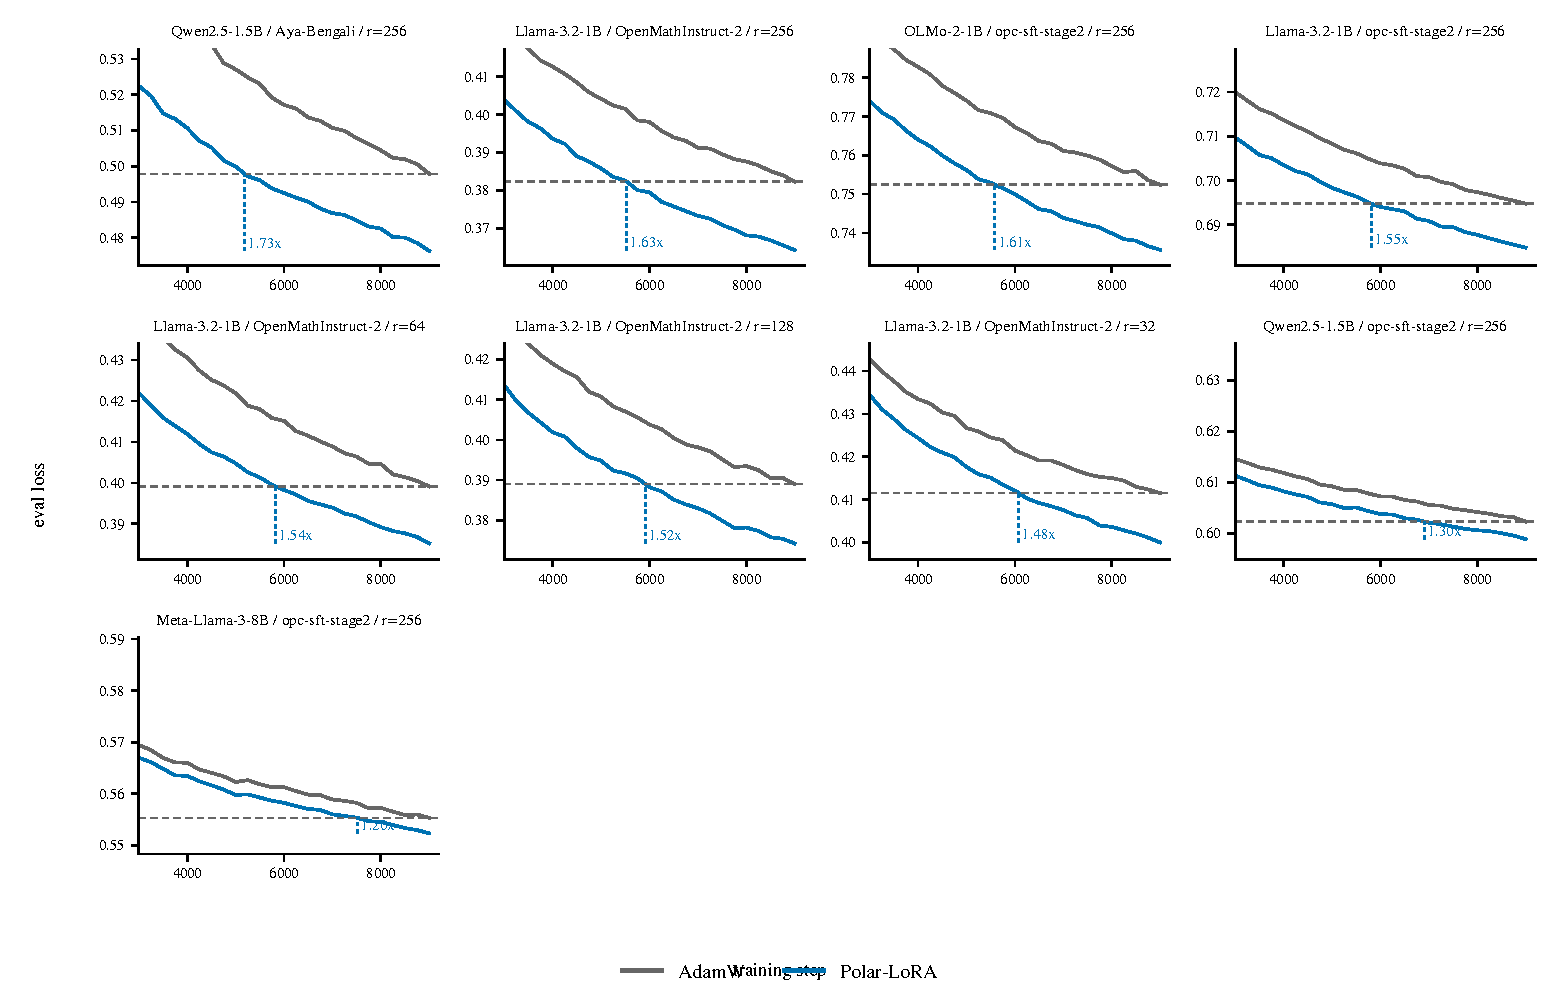
\includegraphics[width=\linewidth]{figA_tailzoom.pdf}
  \caption{\textbf{Tail trajectories per setting.} Eval loss versus step (tail only,
  step $\ge 3000$) for \methodname{} (blue) and AdamW (gray) at each method's best
  learning rate, one panel per setting in \Cref{tab:speedup}. Dashed line: AdamW's
  final loss; the vertical drop-line marks where \methodname{} reaches it, annotated
  with the step speedup. Single seed.}
  \label{fig:tailzoom}
\end{figure}

\printbibliography
\end{document}
